\documentclass[11pt]{article}
\usepackage[a4paper,margin=1in]{geometry}
\usepackage{amsmath,amssymb}
\usepackage{booktabs}
\usepackage{float}
\usepackage{graphicx}
\usepackage{hyperref}
\usepackage{xcolor}
\graphicspath{{figures/}}
\hypersetup{colorlinks=true,linkcolor=blue!45!black,urlcolor=blue!45!black,citecolor=blue!45!black}

\title{Question 4: Regression Control Variates on MCMC Output}
\author{}
\date{}

\begin{document}
\maketitle

\section*{Short answer}

The linear regression step is useful, but it is not an ordinary iid regression.  The rows of the regression matrix are consecutive Metropolis-Hastings draws, so they are autocorrelated.  This means that the usual OLS standard errors, \(p\)-values, and iid variance formulas are not valid.  The estimator itself is still meaningful as an MCMC post-processing estimator, but its numerical error has to be checked with MCMC-aware tools.

This is the point we want to make in the presentation: we should not say ``linear regression is wrong''.  A better statement is: ``the regression coefficient can be estimated from the chain, but we must not pretend the chain gives independent observations''.

\section*{Control-variate regression}

Let \(X_i\) be the post burn-in MCMC draws and let \(f(X_i)\) be the quantity whose posterior mean we want.  In this project, for parameter \(j\),
\[
  f_j(X_i)=\omega_j(X_i).
\]
For the first-order zero-variance control variates of Mira, Solgi and Imparato, we build a vector \(H(X_i)\) such that
\[
  \mathbb E_\pi[H(X)] = 0.
\]
For any fixed coefficient vector \(\beta\),
\[
  \mu
  =
  \mathbb E_\pi[f(X)]
  =
  \mathbb E_\pi[f(X)-H(X)^\top\beta].
\]
The practical estimator is therefore
\[
  \widehat\mu_\beta
  =
  \frac1n\sum_{i=1}^n
  \left\{f(X_i)-H(X_i)^\top\widehat\beta\right\}.
\]
The naive implementation estimates \(\widehat\beta\) by OLS using all MCMC draws and then uses the same draws to estimate the mean.  This is what we compare against three safer variants.

\section*{Why dependence matters}

For an iid regression, the information in \(n\) rows is roughly proportional to \(n\).  In a random-walk Metropolis chain, this is false: if the chain moves slowly, consecutive rows are almost duplicates.  The effective sample size is closer to
\[
  n_{\mathrm{eff}}
  \approx
  \frac{n}{1+2\sum_{k\ge1}\rho_k},
\]
where \(\rho_k\) are autocorrelations.  If these autocorrelations are positive, \(n_{\mathrm{eff}}\ll n\).  That is why a regression fit on MCMC output can look more precise than it really is.

We tested four versions of the zero-variance estimator:
\begin{itemize}
  \item \textbf{ZV naive OLS}: fit the regression and estimate the mean on the same chain;
  \item \textbf{ZV split chain}: fit \(\widehat\beta\) on the first half, estimate the mean on the second half;
  \item \textbf{ZV thinned OLS}: keep only every 8th draw before fitting OLS;
  \item \textbf{ZV block OLS}: average the chain into blocks of size 80, then regress on block means.
\end{itemize}
The split-chain version is conceptually clean because the coefficient fitting sample and the evaluation sample are separated.  Thinning and block averaging are cruder, but they directly attack the dependence problem.

\section*{Small experiment}

The code in \texttt{q4\_mcmc\_regression\_dependence.py} runs 10 independent Metropolis-Hastings chains on simulated GARCH data with
\[
  \omega=(0.2,0.2,0.5),\qquad T=600.
\]
Each chain uses 5000 MH iterations and discards the first 1500 as burn-in.  We then compute the plain MC posterior mean and the four regression-control estimates for each chain.  The numerical error is measured by the empirical variance across the 10 independent chains.

\begin{figure}[H]
  \centering
  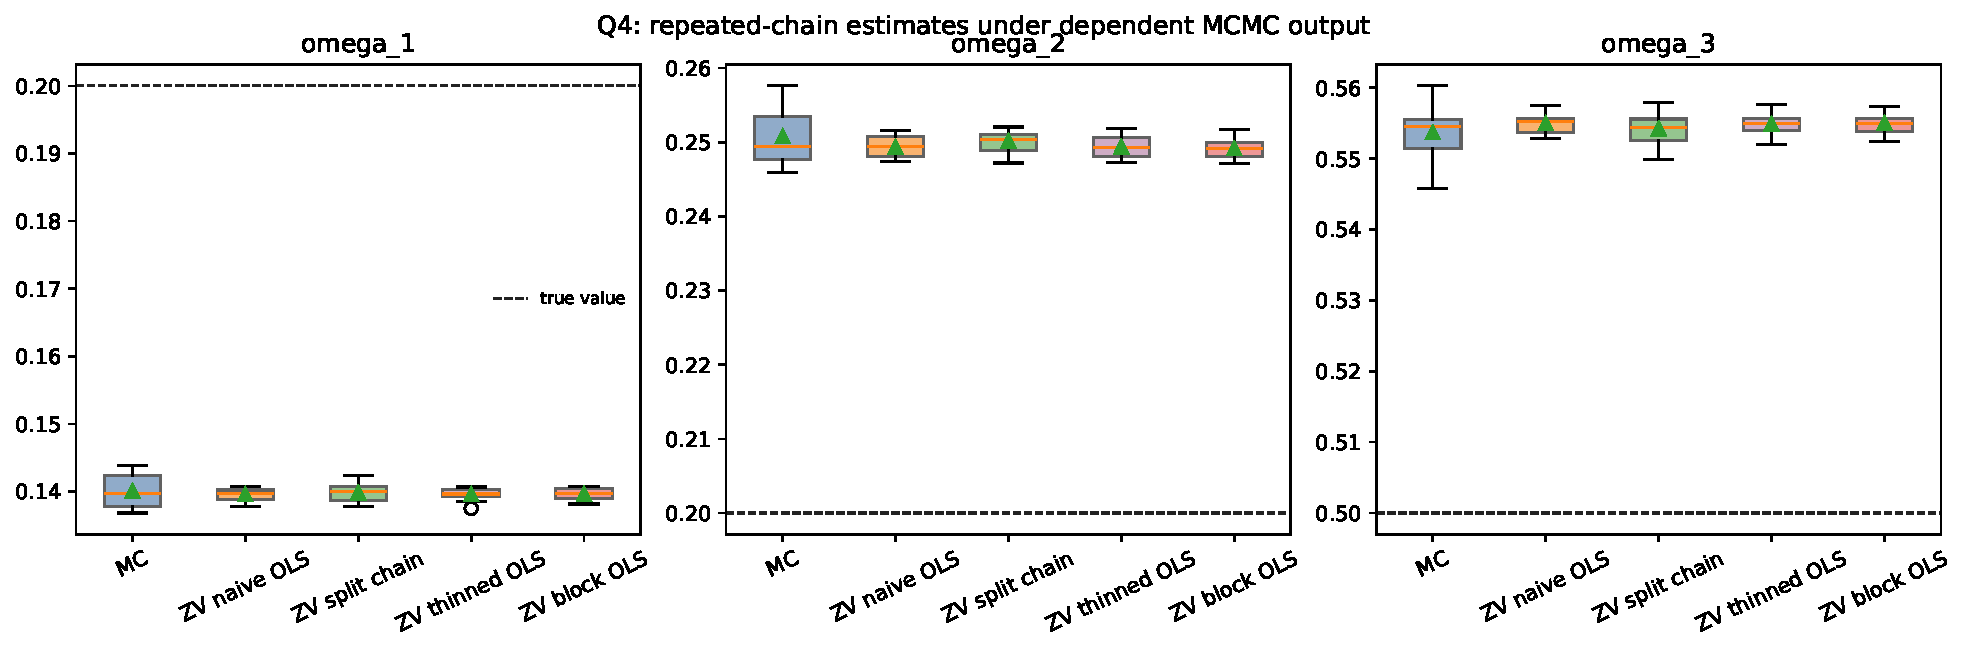
\includegraphics[width=\textwidth]{q4_boxplots.pdf}
  \caption{Repeated-chain estimates.  The dashed line is the data-generating value, used only as a sanity check.  The boxplot width is the important object here: it shows Monte Carlo variability across independent runs.}
\end{figure}

\begin{figure}[H]
  \centering
  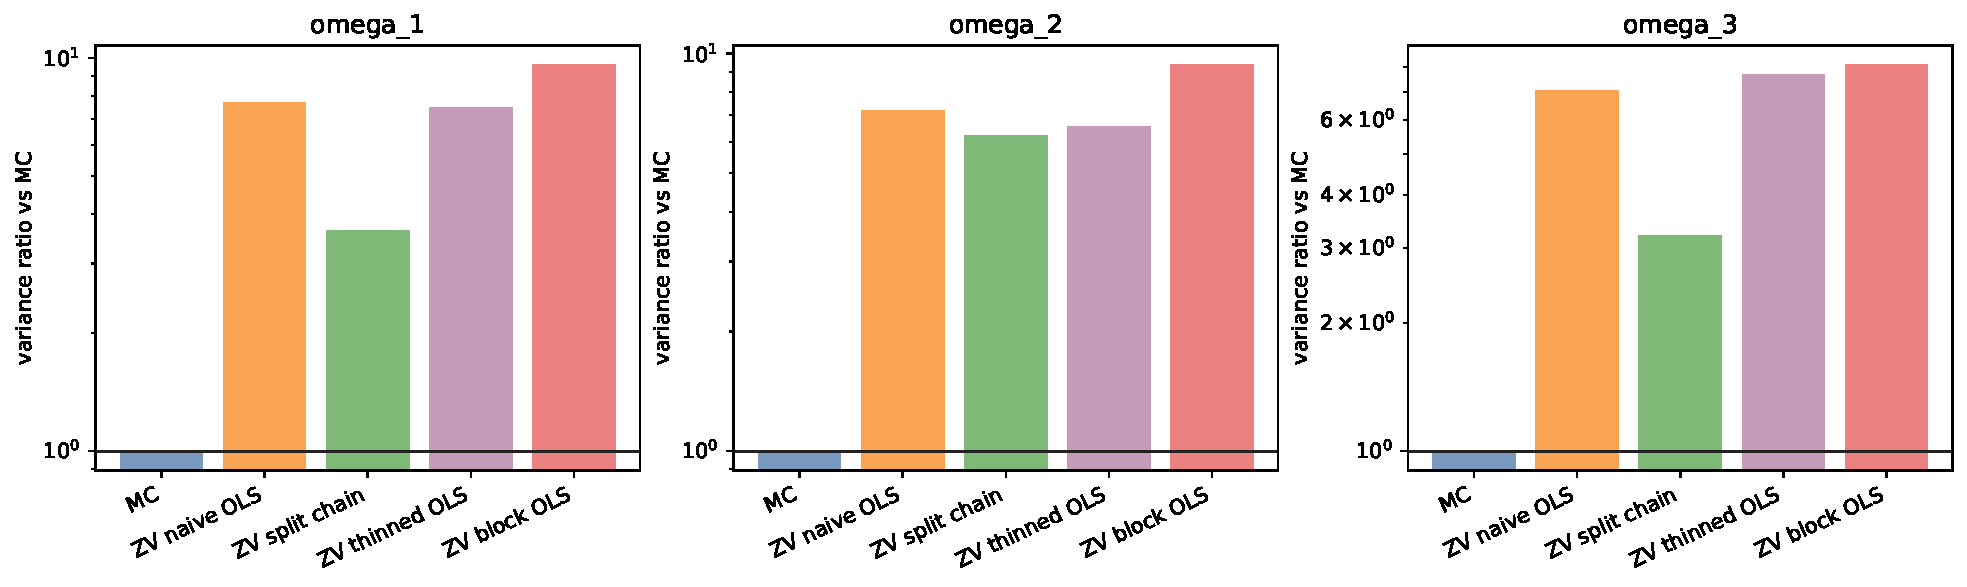
\includegraphics[width=\textwidth]{q4_variance_ratios.pdf}
  \caption{Variance ratio relative to raw Monte Carlo.  Values above 1 mean that the control variate reduced the repeated-chain variance.}
\end{figure}

\begin{figure}[H]
  \centering
  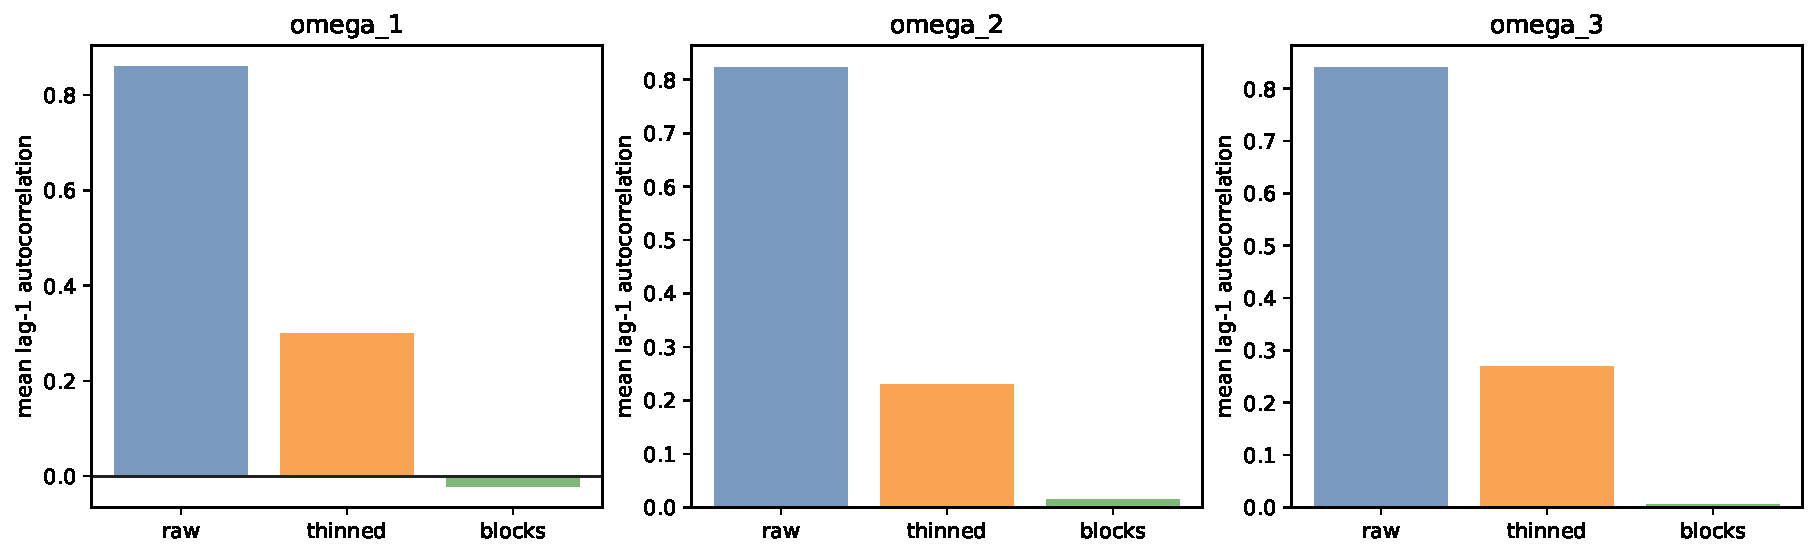
\includegraphics[width=0.9\textwidth]{q4_acf_reduction.pdf}
  \caption{Average lag-1 autocorrelation.  Thinning helps, and block means almost remove lag-1 dependence, but they also use fewer regression rows.}
\end{figure}

\begin{figure}[H]
  \centering
  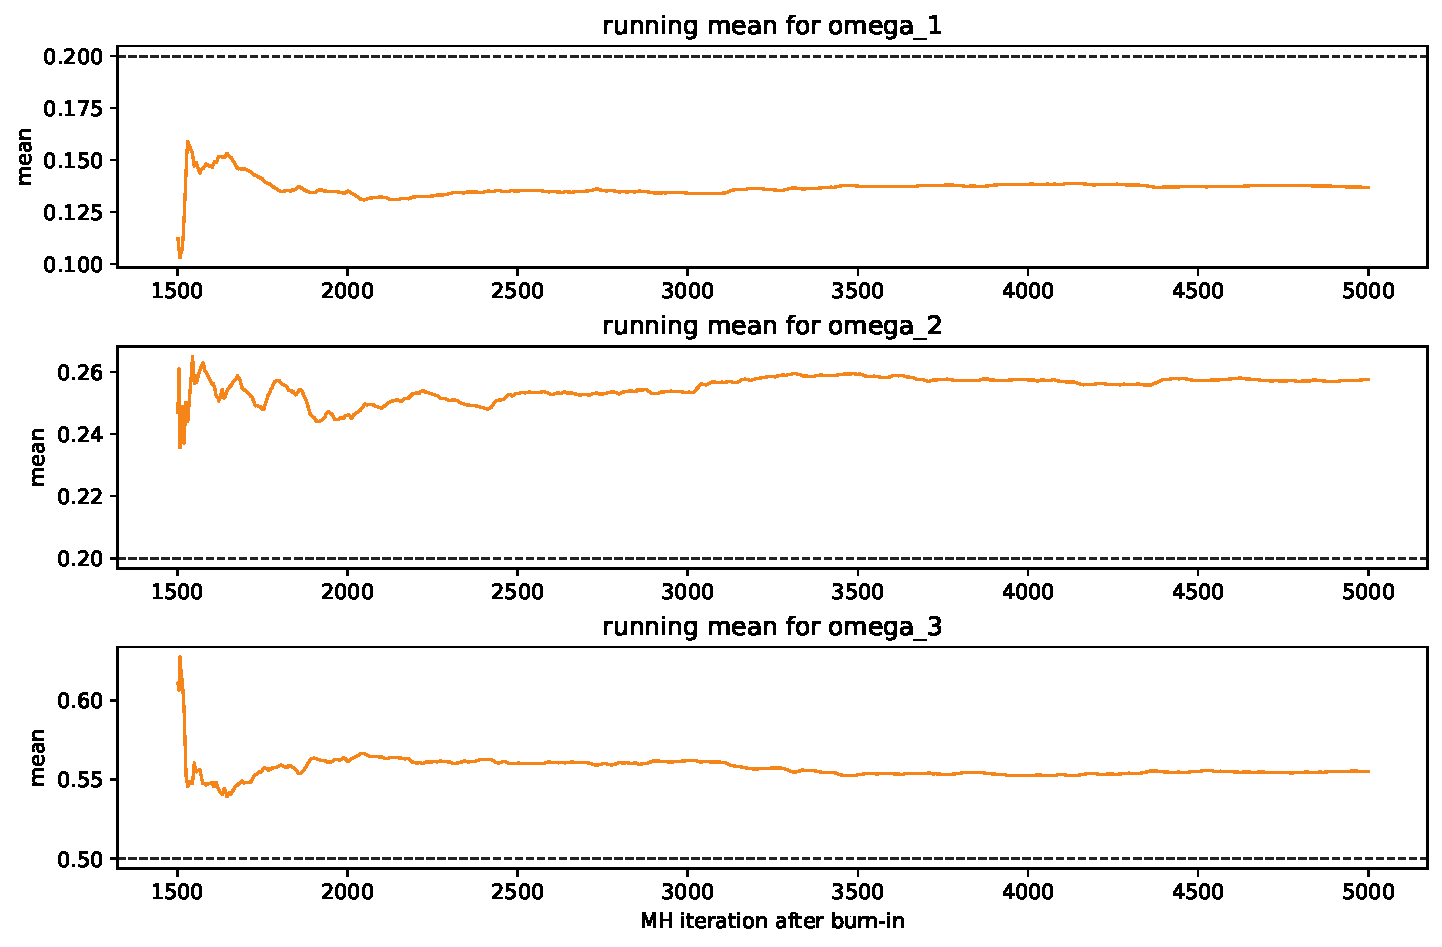
\includegraphics[width=0.85\textwidth]{q4_running_mean.pdf}
  \caption{Running means from one representative chain.  This is a diagnostic plot, not a proof of convergence.}
\end{figure}

\section*{Numerical tables}

\begin{table}[H]
  \centering
  \scriptsize
  \resizebox{\textwidth}{!}{\begin{tabular}{lllllllll}
\toprule
parameter & method & mean\_estimate & variance\_across\_chains & sd\_across\_chains & mean\_batch\_means\_se & mean\_regression\_rows & mc\_variance & variance\_ratio\_vs\_mc \\
\midrule
omega\_1 & MC & 0.1401 & 7.32e-06 & 0.0027 & 0.0025 & 3500.0000 & 7.32e-06 & 1.0000 \\
omega\_1 & ZV block OLS & 0.1396 & 7.63e-07 & 8.73e-04 & 5.67e-04 & 43.0000 & 7.32e-06 & 9.5978 \\
omega\_1 & ZV naive OLS & 0.1396 & 9.50e-07 & 9.75e-04 & 6.51e-04 & 3500.0000 & 7.32e-06 & 7.7015 \\
omega\_1 & ZV split chain & 0.1398 & 2.02e-06 & 0.0014 & 0.0011 & 1750.0000 & 7.32e-06 & 3.6312 \\
omega\_1 & ZV thinned OLS & 0.1396 & 9.78e-07 & 9.89e-04 & 6.57e-04 & 438.0000 & 7.32e-06 & 7.4807 \\
omega\_2 & MC & 0.2508 & 1.64e-05 & 0.0040 & 0.0030 & 3500.0000 & 1.64e-05 & 1.0000 \\
omega\_2 & ZV block OLS & 0.2492 & 1.75e-06 & 0.0013 & 7.78e-04 & 43.0000 & 1.64e-05 & 9.3694 \\
omega\_2 & ZV naive OLS & 0.2494 & 2.28e-06 & 0.0015 & 0.0010 & 3500.0000 & 1.64e-05 & 7.1911 \\
omega\_2 & ZV split chain & 0.2501 & 2.64e-06 & 0.0016 & 0.0016 & 1750.0000 & 1.64e-05 & 6.2116 \\
omega\_2 & ZV thinned OLS & 0.2494 & 2.50e-06 & 0.0016 & 0.0010 & 438.0000 & 1.64e-05 & 6.5579 \\
omega\_3 & MC & 0.5537 & 1.88e-05 & 0.0043 & 0.0045 & 3500.0000 & 1.88e-05 & 1.0000 \\
omega\_3 & ZV block OLS & 0.5550 & 2.32e-06 & 0.0015 & 9.17e-04 & 43.0000 & 1.88e-05 & 8.0926 \\
omega\_3 & ZV naive OLS & 0.5550 & 2.67e-06 & 0.0016 & 0.0011 & 3500.0000 & 1.88e-05 & 7.0357 \\
omega\_3 & ZV split chain & 0.5542 & 5.84e-06 & 0.0024 & 0.0018 & 1750.0000 & 1.88e-05 & 3.2118 \\
omega\_3 & ZV thinned OLS & 0.5549 & 2.44e-06 & 0.0016 & 0.0011 & 438.0000 & 1.88e-05 & 7.6929 \\
\bottomrule
\end{tabular}
}
  \caption{Repeated-chain variance comparison for Q4.  The column \texttt{variance\_ratio\_vs\_mc} is the variance of raw MC divided by the variance of the method.}
\end{table}

\begin{table}[H]
  \centering
  \small
  \resizebox{\textwidth}{!}{\begin{tabular}{llll}
\toprule
parameter & series & mean\_lag1\_acf & sd\_lag1\_acf \\
\midrule
omega\_1 & block means size 80 & -0.0214 & 0.1589 \\
omega\_1 & raw chain & 0.8601 & 0.0146 \\
omega\_1 & thinned every 8 & 0.2990 & 0.0507 \\
omega\_2 & block means size 80 & 0.0142 & 0.0907 \\
omega\_2 & raw chain & 0.8230 & 0.0094 \\
omega\_2 & thinned every 8 & 0.2292 & 0.0482 \\
omega\_3 & block means size 80 & 0.0049 & 0.1709 \\
omega\_3 & raw chain & 0.8406 & 0.0215 \\
omega\_3 & thinned every 8 & 0.2682 & 0.0731 \\
\bottomrule
\end{tabular}
}
  \caption{Lag-1 autocorrelation summary.  Blocks make the regression rows much less dependent, at the price of fewer rows.}
\end{table}

\section*{Conclusion for the oral presentation}

The answer to the bonus question is: not completely.  The OLS projection idea is fine as a variance-reduction device, but the iid regression interpretation is not valid on an MCMC chain.  In our results, the zero-variance estimators still reduce variance by a large factor compared with raw MC.  However, the safer variants are easier to defend: split-chain regression avoids using exactly the same draws for fitting and evaluation, while thinning and block averaging reduce the visible dependence in the regression design.

So the practical recommendation is to report repeated independent-chain boxplots, and if we use regression control variates, also report a dependence-aware check such as split-chain, thinning, block means, or batch-means standard errors.

\begin{thebibliography}{9}
\bibitem{mira2013}
A. Mira, R. Solgi, and D. Imparato.
\newblock Zero variance Markov chain Monte Carlo for Bayesian estimators.
\newblock \emph{Statistics and Computing}, 23, 653--662, 2013.

\bibitem{geyer1992}
C. J. Geyer.
\newblock Practical Markov Chain Monte Carlo.
\newblock \emph{Statistical Science}, 7(4), 473--483, 1992.
\end{thebibliography}

\end{document}
